%%%%%%%%%%%%%%%%%%%%%%%%%%%%%%%%%%%%%%%%%%%%%%%%%%%%%%%%%%%%%%%%%%%%%%%%%%%%
% AGUJournalTemplate.tex: this template file is for articles formatted with LaTeX
%
% This file includes commands and instructions
% given in the order necessary to produce a final output that will
% satisfy AGU requirements, including customized APA reference formatting.
%
% You may copy this file and give it your
% article name, and enter your text.
%
% guidelines and troubleshooting are here: 

%% To submit your paper:
\documentclass[draft]{agujournal2019}
\usepackage{url} %this package should fix any errors with URLs in refs.
\usepackage{lineno}
\usepackage[inline]{trackchanges} %for better track changes. finalnew option will compile document with changes incorporated.
\usepackage{soul}
\linenumbers
%%%%%%%
% As of 2018 we recommend use of the TrackChanges package to mark revisions.
% The trackchanges package adds five new LaTeX commands:
%
%  \note[editor]{The note}
%  \annote[editor]{Text to annotate}{The note}
%  \add[editor]{Text to add}
%  \remove[editor]{Text to remove}
%  \change[editor]{Text to remove}{Text to add}
%
% complete documentation is here: http://trackchanges.sourceforge.net/
%%%%%%%

\draftfalse

%% Enter journal name below.
%% Choose from this list of Journals:
%
% JGR: Atmospheres
% JGR: Biogeosciences
% JGR: Earth Surface
% JGR: Oceans
% JGR: Planets
% JGR: Solid Earth
% JGR: Space Physics
% Global Biogeochemical Cycles
% Geophysical Research Letters
% Paleoceanography and Paleoclimatology
% Radio Science
% Reviews of Geophysics
% Tectonics
% Space Weather
% Water Resources Research
% Geochemistry, Geophysics, Geosystems
% Journal of Advances in Modeling Earth Systems (JAMES)
% Earth's Future
% Earth and Space Science
% Geohealth
%
% ie, \journalname{Water Resources Research}

\journalname{JGR: Planets}


\begin{document}

%%%%%%%%%%%%%%%%%%%%%%%%%%%%%%%%%%%%%%%%%%%%%%%
%  TITLE
%
% (A title should be specific, informative, and brief. Use
% abbreviations only if they are defined in the abstract. Titles that
% start with general keywords then specific terms are optimized in
% searches)
%
%%%%%%%%%%%%%%%%%%%%%%%%%%%%%%%%%%%%%%%%%%%%%%%

% Example: \title{This is a test title}

\title{Aerosols in the vacuum: modelling the time variability of the plume of Enceladus}

%%%%%%%%%%%%%%%%%%%%%%%%%%%%%%%%%%%%%%%%%%%%%%%
%
%  AUTHORS AND AFFILIATIONS
%
%%%%%%%%%%%%%%%%%%%%%%%%%%%%%%%%%%%%%%%%%%%%%%%

% Authors are individuals who have significantly contributed to the
% research and preparation of the article. Group authors are allowed, if
% each author in the group is separately identified in an appendix.)

% List authors by first name or initial followed by last name and
% separated by commas. Use \affil{} to number affiliations, and
% \thanks{} for author notes.
% Additional author notes should be indicated with \thanks{} (for
% example, for current addresses).

% Example: \authors{A. B. Author\affil{1}\thanks{Current address, Antartica}, B. C. Author\affil{2,3}, and D. E.
% Author\affil{3,4}\thanks{Also funded by Monsanto.}}

\authors{=list all authors here=}


% \affiliation{1}{First Affiliation}
% \affiliation{2}{Second Affiliation}
% \affiliation{3}{Third Affiliation}
% \affiliation{4}{Fourth Affiliation}

\affiliation{=number=}{=Affiliation Address=}
%(repeat as many times as is necessary)


% Corresponding author mailing address and e-mail address:

% (include name and email addresses of the corresponding author.  More
% than one corresponding author is allowed in this LaTeX file and for
% publication; but only one corresponding author is allowed in our
% editorial system.)

% Example: \correspondingauthor{First and Last Name}{email@address.edu}

\correspondingauthor{=name=}{=email address=}



%%%%%%%%%%%%%%%%%%%%%%%%%%%%%%%%%%%%%%%%%%%%%%%
% KEY POINTS
%%%%%%%%%%%%%%%%%%%%%%%%%%%%%%%%%%%%%%%%%%%%%%%
%  List up to three key points (at least one is required)
%  Key Points summarize the main points and conclusions of the article
%  Each must be 140 characters or fewer with no special characters or punctuation and must be complete sentences

% Example:
% \begin{keypoints}
% \item	List up to three key points (at least one is required)
% \item	Key Points summarize the main points and conclusions of the article
% \item	Each must be 140 characters or fewer with no special characters or punctuation and must be complete sentences
% \end{keypoints}

\begin{keypoints}
\item A one dimensional model couples liquid level gas flow and wall heat diffusion in a tidally flexing south polar crack on Enceladus
\item Diurnal widening and narrowing of the crack drives the water level up and down and modulates the water vapor mass flux of the plume
\item Heat stored in a thin wall layer produces a secondary plume peak near mean anomaly fifty degrees consistent with observations
\end{keypoints}

%%%%%%%%%%%%%%%%%%%%%%%%%%%%%%%%%%%%%%%%%%%%%%%
%
%  ABSTRACT and PLAIN LANGUAGE SUMMARY
%
% A good Abstract will begin with a short description of the problem
% being addressed, briefly describe the new data or analyses, then
% briefly states the main conclusion(s) and how they are supported and
% uncertainties.

% The Plain Language Summary should be written for a broad audience,
% including journalists and the science-interested public, that will not have 
% a background in your field.
%
% A Plain Language Summary is required in GRL, JGR: Planets, JGR: Biogeosciences,
% JGR: Oceans, G-Cubed, Reviews of Geophysics, and JAMES.
% see http://sharingscience.agu.org/creating-plain-language-summary/)
%
%%%%%%%%%%%%%%%%%%%%%%%%%%%%%%%%%%%%%%%%%%%%%%%

%% \begin{abstract} starts the second page

\begin{abstract}
Previous studies have examined the dynamics of water vapor arising from liquid water in the cracks near the south pole of Enceladus \cite{nimmo2007shear,Schmidt2008,ingersoll2010subsurface,postberg2011salt,nimmo2014tidally,kite2016sustained,nakajima2016controlled}. In this work, we present a model in which the water level rises and falls due to the diurnal widening and narrowing of the walls. We also consider sublimation from the walls as they are periodically covered and uncovered by liquid water. The observed plume activity has a main peak near mean anomaly (MA) of 180 degrees and a secondary peak near MA of 50 degrees \cite{hedman2013observed,ingersoll2020time,nimmo2014tidally}, the latter occurring only over a narrow range of crack widths. We show that this narrow-width regime is not a fine-tuned coincidence but an attractor: because the water level is highly sensitive to the crack width, and because the plume continuously condenses ice back onto the walls and seals the crack, any crack that flexes at all is driven within a few diurnal cycles --- regardless of its initial size --- toward a small-width state in which the water reaches the surface and produces the secondary peak. The absolute tidal swing of the walls, rather than acting as a threshold, sets only how far the crack must seal before it overflows. The rising water keeps the vent open against the rapid condensation, sustaining a two-way exchange of water between the oxidizing surface and the reducing ocean that is relevant to the habitability of Enceladus \cite{parkinson2008habitability}.
\end{abstract}

\section*{Plain Language Summary}
Enceladus, an icy moon of Saturn, sprays jets of water vapor and ice grains into space from warm cracks near its south pole. The brightness of these plumes rises and falls over each 33-hour orbit, with a strong peak and a weaker secondary peak at a specific point in the orbit. We build a simple physical model of a single crack whose walls are squeezed and stretched by Saturn's tides, causing liquid water inside to rise and fall like a piston. The narrower the crack, the higher the water is driven. We find that the escaping vapor continually freezes back onto the walls and narrows the crack, and that this self-sealing acts as a trap: whatever its starting width, any crack that flexes with the tides is squeezed within days to a narrow state in which the water reaches the surface and erupts, producing the secondary brightening. The rising water keeps the vent from freezing shut, sustaining an exchange of water between the surface and the buried ocean that matters for the moon's potential to support life.


%%%%%%%%%%%%%%%%%%%%%%%%%%%%%%%%%%%%%%%%%%%%%%%
%
%  BODY TEXT
%
%%%%%%%%%%%%%%%%%%%%%%%%%%%%%%%%%%%%%%%%%%%%%%%

%%% Suggested section heads:
% \section{Introduction}
%
% The main text should start with an introduction. Except for short
% manuscripts (such as comments and replies), the text should be divided
% into sections, each with its own heading.

% Headings should be sentence fragments and do not begin with a
% lowercase letter or number. Examples of good headings are:

% \section{Materials and Methods}
% Here is text on Materials and Methods.
%
% \subsection{A descriptive heading about methods}
% More about Methods.
%
% \section{Data} (Or section title might be a descriptive heading about data)
%
% \section{Results} (Or section title might be a descriptive heading about the
% results)
%
% \section{Conclusions}

\section{Introduction}
In 2005, the Cassini spacecraft found a geologically active south pole on Saturn’s moon Enceladus \cite{porco2006cassini}. Plumes that contain vapor and icy particles were identified and were considered to supply Saturn’s E-ring. The plumes emanate from four major fractures that sum up to about 500 km in length, and their locations agree well with the hotspots identified in infrared images \cite{spitale2007association}. The analysis of the Cassini Ultraviolet Imaging Spectrograph (UVIS) data in solar occultation reveals that the total rate of emission of water vapor from the surface is 200~400 kg/s \cite{hansen2011composition, hansen2017investigation}. Data from the Cosmic Dust Analyzer (CDA) and the Ion and Neutral Mass Spectrometer (INMS) revealed macromolecular organic compounds in the icy grains \cite{postberg2018macromolecular}. Being a region with far more infrared emission than other parts of the planet, the value of the non-solar radiated power from the south polar region ranges from 4.2 GW \cite{spencer2013enceladus} and 5.8$\pm$1.9GW \cite{spencer2006cassini} to 15.8$\pm$3.1GW \cite{howett2011high}.

By observing the details of the plume structures and compositions, the ice/vapor ratio is estimated to be 0.35~0.70, indicating that a liquid reservoir might be the source of the plumes \cite{ingersoll2011total}. Further studies that reveal the existence of salt-rich ice grains and organic compounds in the plumes increased the confidence that the plumes originated from a liquid source \cite{postberg2018macromolecular}. It has been confirmed later that the amplitude of the forced libration of Enceladus is too large for a model in which the icy crust is rigidly connected with its rocky core \cite{thomas2016enceladus}. This implies the presence of a global ocean on Enceladus. If the tiger stripes are considered strike-slip faults, the shear heating would be sufficient to support the existence of liquid water in the cracks \cite{parkinson2008habitability}. If two walls are decoupled and form a water-filled crack, the turbulent dissipation could supply the observed amount of heat emission from the south pole \cite{kite2016sustained}. 

Our goal is to further understand the dynamics and time variability of the plumes, as shown in Fig. \ref{fig:enc:1}. The plume brightness, which is related to the abundance of micron-sized particles, is 4-5 times greater at the apocenter than at the pericenter. The maximum occurs about 20 degrees in orbital phase after the apocenter. A secondary maximum occurs about 40 degrees after the pericenter \cite{hedman2013observed,ingersoll2017decadal}. The variability is thought to be evidence of the opening and closing of the cracks due to the eccentricity tide, potentially with a physical libration and a viscoelastic interior \cite{hurford2007eruptions,nimmo2014tidally}. The timing of the plume eruptions has also received explanations from a specific interior viscosity structure \cite{bvehounkova2017plume}.

\begin{figure}[hbt!]
    \centering
    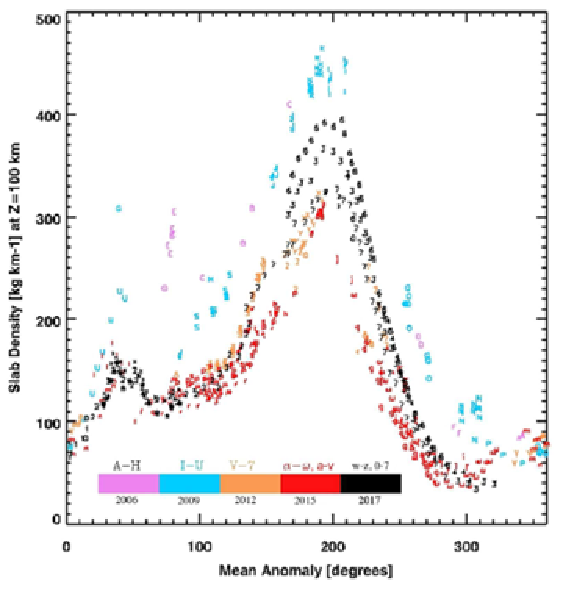
\includegraphics[width=0.5\textwidth]{Figures/Figure_1.pdf}
    \caption{Slab density vs mean anomaly, adapted from \citeA{ingersoll2020time}. The data are grouped in three-year intervals and show a distinct secondary peak at around MA 50 degrees. Slab density is the mass of ice particles per unit thickness of a horizontally infinite slab above the south pole. The figure shows slab density at 100 km altitude. It is derived from the observed brightness using a model of how the particles scatter light.}
    \label{fig:enc:1}
\end{figure}

In this paper, we focus on the secondary peak observed as shown in Fig. \ref{fig:enc:1} \cite{hedman2013observed,ingersoll2020time,nimmo2014tidally}, and use the rise and fall of the water as an indic of two-way mass transfer between surface and ocean. We present the configuration of the model and the simulation results and make comparisons with the observations.

The thermal coupling between the liquid water and the walls was previously modeled by considering the turbulent dissipation of water as it moved up and down in response to the widening and narrowing of the cracks \cite{kite2016sustained}. Changes in the height of the liquid-gas interface were noted but not included in their discussion of heat dissipation. We show that water level changes are important only when the mass of the plumes is considered. Such rising and falling of the water level come from vertical pressure gradients, one due to the inertia of the fluid and the other due to friction with the walls.

\section{Methods}
In this work, we use a one-dimensional model to study how the mass flux changes during one period of Enceladus’ rotation. The novelty of our model is the rising and falling of the water level, together with its associated effects. \citeA{nakajima2016controlled} suggested a controlled boiling model, which describes a mechanism of the plume evaporating from the gas-liquid interface held near 273 K and the fluid dynamics of the gas and liquid in the crack (regions 2 and 4 in Fig. \ref{fig:enc:2}). Our work also solves the time-dependent heat equation for a thin layer (region 5) at the walls: As the water rises and the wall is covered by water, it absorbs heat by conduction, and when the water level falls and the wall is exposed, it releases heat by sublimation. The time-averaged net heat due to condensation on the walls is conducted through the ice in region 3 and ultimately radiated to space in region 1.
\begin{figure}[hbt!]
    \centering
    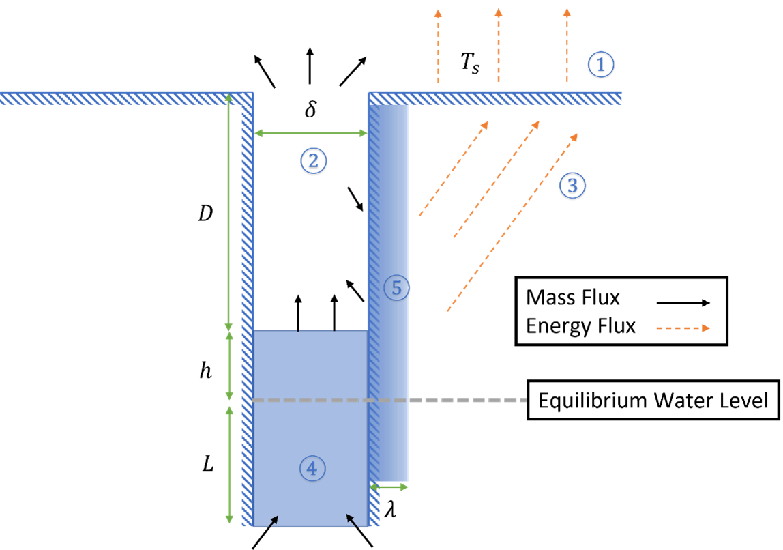
\includegraphics[width=0.7\textwidth]{Figures/Figure_2.pdf}
    \caption{Illustration of the problem. Different regions are denoted by numbers in the circles, while the interactions between regions are denoted by arrows.}
    \label{fig:enc:2}
\end{figure}

We assume a sinusoidal time dependence of crack width, with a minimum at the phase of 0 degrees and a maximum at the phase of 180 degrees, as in Equation \ref{Eq: Enceladus-1}.

\begin{equation}
    \delta(t)=\delta_{min}\left(\frac{R_\delta+1}{2}-\frac{R_\delta-1}{2}\cos\frac{2\pi t}{P}\right)
    \label{Eq: Enceladus-1},
\end{equation}

Here $t$ is the time where the model phase is at 0 degrees, $\delta(t)$ is the crack width, $\delta_{min}$ is the smallest width, and $R_\delta$ is the ratio of the maximum width to the smallest. $P$ is 33 hours, the period of Enceladus' rotation and revolution, being the same as it is tidally locked.
\textbf{However, it may be more appropriate to use a double-cosine when considering tidally-heated processes as described in \citeA{MeyerZuWestram2024}. In this way, one can rewrite Eqn. \ref{Eq: Enceladus-1} with the identity:} \[
\cos\phi = \frac{4}{3}\cos\phi - \frac{1}{3}\cos 2\phi + \frac{1}{3}
\]

\textbf{so that: }

\begin{equation}
\delta(t) = \delta_{\min} \left( \frac{R_\delta + 1}{3} - \frac{2(R_\delta-1)}{3} \cos\frac{2\pi t}{P} + \frac{R_\delta-1}{6} \cos\frac{4\pi t}{P} \right)
\end{equation}




In Fig. \ref{fig:enc:1}, $L$ is the equilibrium depth of the liquid water column, $h$ is the water level height above the neutral water level, $D$ is the instantaneous depth of the water level, and the height $z$ is set to be zero at the bottom of the crack (where it connects to an ocean) and increases upwards. With the walls widening and narrowing, the liquid water moves vertically, and its velocity is a function of both time and height, $v=v(z,t)$. For convenience, we denote the velocities at the entrance of the crack and the gas-liquid interface as $v_0=v(0,t)$ and $v_h=v(h+L,t)$, respectively.

\subsection{Fluid dynamics of the liquid}
In this part of the model, the two dependent variables are the velocity of the water $v_0$ at the entrance of the crack and the water level height $h$. These variables are functions of time and are solved from equations of continuity and momentum. Inertial, gravitational, and frictional forces are applied to the liquid water column.

The velocities at other locations are calculated from continuity by
\begin{equation}
    v(z,t)=v_0(t)-\frac{1}{\delta}\frac{d\delta}{dt}z, 0\leq z \leq h+L.
    \label{Eq: Enceladus-2}
\end{equation}

The time derivative of the entrance velocity is calculated from the momentum equation
\begin{equation}
    \rho_w \delta \frac{\partial v}{\partial t} = -\rho_w \delta v \frac{\partial v}{\partial z} - \delta \frac{\partial p}{\partial z} - \delta \rho_w g - f \hat{v},
    \label{Eq: Enceladus-3}
\end{equation}

Here $g=0.113$ m$^2$s$^{-1}$ is the gravitational acceleration, $f$ is the magnitude of the friction force, and $\hat{v}$ is the sign of the velocity. The time derivative of the entrance velocity at the base of the crack is calculated by substituting Equation \ref{Eq: Enceladus-2} into Equation \ref{Eq: Enceladus-3} and integrating from $z = 0$ to $z = h + L$, assuming that the bottom of the crack has a fixed hydrostatic pressure of $gL$:
\begin{equation}
    \frac{dv_0}{dt} = \frac{1}{h+L} \left[ -\frac{1}{2} \left( v_h^2 - v_0^2 \right)
- \frac{1}{2} \left[ \left( \frac{d\delta}{dt} \right)^2 \frac{1}{\delta^2} - \frac{d^2\delta}{dt^2} \frac{1}{\delta} \right] (h+L)^2
- gh - \int_0^{h+L} \frac{2C_f}{\delta} v^2 \hat{v} \, dz \right].
\label{Eq: Enceladus-4}
\end{equation}
Here $v_h$ is the velocity at the top of the liquid, or the velocity at $z=h+L$. The first two terms on the right-hand side of Equation \ref{Eq: Enceladus-4} are from the advection term in Equation \ref{Eq: Enceladus-3}; the third term is from the gravitational force; and the last term is from the friction force with the two walls. The magnitude of the frictional stress on each wall is calculated as
\begin{equation}
    f=C_f\rho_w v^2,
\end{equation}

where $\rho_w=1000$ kg/m$^3$ is the density of liquid water. The Fanning friction coefficient $C_f$ is not held fixed but is evaluated at the local Reynolds number $Re = \rho_w |v| D_h / \mu$ (hydraulic diameter $D_h = 2\delta$, dynamic viscosity $\mu = 1.8\times10^{-3}$~Pa\,s) using the single-equation correlation of \citeA{churchill1977}, which blends the laminar limit $C_f = C_{\rm lam}/(8\,Re)$ (with $C_{\rm lam}=96$ for an infinite parallel-plate gap) and the turbulent regime smoothly across all flow regimes (following \citeA{ingersoll2010subsurface,arya2001introduction}). The appearance of $\hat{v}$ in Equations \ref{Eq: Enceladus-3} and \ref{Eq: Enceladus-4} shows that the direction of the friction force is opposite to the local velocity direction as given in Equation \ref{Eq: Enceladus-1}. For the smallest width considered in this work, the effect of surface tension is 4 orders of magnitude smaller than the gravitational effect of a 1-meter thick water column and hence is not considered in Equation \ref{Eq: Enceladus-4}.

The time derivative of $h$ is the velocity at location $h+L$ and is obtained from Equation \ref{Eq: Enceladus-2}

\begin{equation}
    \frac{dh}{dt} = v(h+L,t) = v_0 - \frac{h+L}{\delta} \frac{d\delta}{dt}.
\label{Eq: Enceladus-6}
\end{equation}

Equations \ref{Eq: Enceladus-4} and \ref{Eq: Enceladus-6} are the non-linear, time-dependent equations for the dependent variables $v_0(t)$ and $h(t)$. Detailed derivations can be found in Supporting Information.

\begin{equation}
    \frac{dM}{M} (1 - M^2) \left( 1 + \frac{\gamma - 1}{2} M^2 \right)^{-1} = \left( \frac{E}{\rho v \delta} + \frac{\gamma C_f}{2\delta} M^2 \right) dz.
\end{equation}

\subsection{Heat storage and evaporation}
\label{sec:heat}
The heat transfer in the thin layer of the wall (region 5) is controlled by two processes: heat conduction (region 3) and sublimation/condensation of the water vapor (region 2). The two processes differ greatly in their characteristic time scale. Region 5 serves as a thermal conduction layer that connects the two parts of the model. It has a thickness of 1 meter, which is several times the thermal skin depth corresponding to the time of a diurnal cycle ($\sim$0.33 m). This thickness allows us to resolve most of the variabilities associated with a diurnal cycle.

A section of the wall is covered for part of the diurnal cycle, and the wall absorbs heat from the water when it is submerged. When the water level falls, these sections of the wall are exposed and the water vapor either evaporates from or condenses onto the exposed walls. The sublimation rate (negative if condensation) per unit area of an exposed wall is calculated as
\begin{equation}
    E(z,t) = \frac{p_w(z,t) - p_g(t)}{\sqrt{2\pi R T_w(z,t)}},
\end{equation}
Where $p_g(t)$ is the pressure of the gas at region 2 at time $t$, $p_w(z,t)$ is the saturated vapor pressure for the wall at height $z$ and time $t$, and $T_w(z,t)$ is the temperature of the wall at height
$z$ and time $t$.

We name the two boundaries of the thermal layer (region 5) as the sublimation-side boundary (interface with regions 2 and 4) and conduction-side boundary (interface with region 3), respectively. The evaporation-side boundary of the shallow layer is set to have a temperature gradient pertinent to the rate of condensation or sublimation at the wall surface.

The saturated vapor pressure is obtained to a good approximation from $p_w=A\exp\left(-B/T_w\right)$ where $A=3.63\times 10^{12}$ Pa and $B=6147$ K \cite{nakajima2016controlled}.

At the surface (region 1), the heat release is controlled by blackbody radiation, and within the ice crust (region 3) steady-state heat conduction happens \cite{ingersoll2010subsurface}, as in Equation
\ref{Eq: Enceladus-8}. Here $T_s(d)$ is the temperature of the surface with a horizontal distance $d$ from the crack, and $\lambda$ is the thickness of the thermal layer, or region 5. The conduction-side boundary of the thermal layer is set to match the steady-state heat conduction in region 3 at the boundary with region 5.

\begin{eqnarray}
    F_c = 4k \frac{T_s(d) - T(z,\lambda,t)}{\pi d}.
\label{Eq: Enceladus-8}
\end{eqnarray}

Eaccrack has two walls, one on either side. Details of the heat transfer are shown in Supporting Information.

\subsection{Fluid dynamics of the gas}
The gas dynamics (region 2) are described by a model that is similar to that in \citeA{nakajima2016controlled}. However, the sublimation and condensation happening on the surface of the walls (region 5) are treated differently, as we are now solving a transient state. Similar to \citeA{nakajima2016controlled}, the flow is initialized with evaporation at the liquid surface and travels upwards. Besides the thermodynamic variables pressure and temperature, and the vertical velocity of the gas, we keep track of the Mach number by integrating from the gas-liquid interface to the exit of the crack:
\begin{equation}
    \frac{dM}{M} (1 - M^2) \left( 1 + \frac{\gamma - 1}{2} M^2 \right)^{-1} = \left( \frac{E}{\rho v \delta} + \frac{\gamma C_f}{2\delta} M^2 \right) dz
    \label{Eq: Enceladus-9}.
\end{equation}
Noticeably, the Mach number condition $M=1$ at the exit is the physical limit of the compressible flow in a frictional duct, which is the physical constraint used in \citeA{nakajima2016controlled}. However, from Equation \ref{Eq: Enceladus-9}, we note that in the presence of mass removal ($E<0$), the Mach number is allowed to exceed 1. Hence, we use a different exit boundary condition here.

According to \citeA{dong2011water}, the best-fit exit Mach number of the plume is 1.4-1.8. The slight difference could be due to the expansion and acceleration near the exit of the crack. Also, we confirmed with simulations that the boundary mach number has a minimal effect on the mass flux in the range of 1.4-1.8. Hence, we use $M=1.6$ here as the exit condition. Also, most of the conclusions in \citeA{nakajima2016controlled} still hold: having Mach numbers of 1.4 or 1.8 as the exit condition creates a total mass flux difference of no more than 2\% for shell thickness of 5 km and 5\% for shell thickness of 20 km. The details of the derivation of Equation \ref{Eq: Enceladus-9} can be found in Supporting Information. 

Different parts are assembled into a full model. The rising of falling of water level is solved first, which is used for calculation of the mass flux. To model the variability of the mass flux, we need to solve for the flow of water vapor. The water level is evaporative, creating a flow in the crack, but the mass flux and the speed of the initiated flow depends on the initial water vapor back pressure $p_b$ just above the water level. The flow accelerates and exchanges mass with the walls, and the value of $p_b$ is iteratively selected to match the condition that $M=1.6$ at the exit. The model is run for about 100 days on Enceladus until the diurnal oscillations in the thermal layer stabilize. 

\section{Results}
To explore the effects of each parameter, we conducted simulations on a parameter grid. The three controlling parameters are the equilibrium water column depth $L$, the minimum width $\delta_{min}$ and the ratio of the maximum width to the minimum width $R_{\delta}$ The selections of the parameters are specified in Table \ref{tbl:enc:model_parameters}. For the choices of minimum width values, we selected a wide range ranging from centimeters suggested by \citeA{nakajima2016controlled} to a meter suggested by \citeA{kite2016sustained}. As shown below, the self-sealing feedback drives cracks across this entire range toward a common small-width state, so the relevant behavior is set not by the initial width but by the width ratio $R_\delta$ and depth $L$.

\begin{table}[hbt!]
    \centering
    \begin{tabular}{l l}
        \hline
        \textbf{Parameter} & \textbf{Choices of values} \\
        \hline
        Equilibrium water depth $L$ & 5 km, 10 km, and 20 km \\
        Minimum width $\delta_{min}$ & 1 mm, 2 mm, 5 mm, 1 cm, 5 cm, 20 cm, 50 cm, 1 m \\
        Width ratio $R_\delta$ & 1.05, 1.0, 1.15, 1.2, 1.3, 1.5, 2.0, 3.0, 5.0 \\
        \hline
    \end{tabular}
    \caption{Parameters selected for model simulations.}
    \label{tbl:enc:model_parameters}
\end{table}

We study how the water level responds to the wall motion; this response is what the self-sealing feedback of Section~\ref{sec:attractor} acts upon.

\subsection{Water level variation}
The diurnal cycle decomposes into an expanding phase (MA 0--180$^\circ$) and a squeezing phase (MA 180--360$^\circ$). When the walls expand, the water level first drops by continuity and is then refilled by gravity; when the walls squeeze, the water is driven upward and falls back once the level is high. The minimum width $\delta_{min}$ sets the amplitude of this excursion through friction: a narrower crack forces the water faster and traps more of it, producing a larger rise.

This sensitivity can be captured analytically. The in-crack velocity scales as $(1/\delta)(d\delta/dt)$ and the wall friction as $(1/\delta)^2(d\delta/dt)^2$; with $d\delta/dt\propto\delta R_\delta$, the maximum water-level rise scales as
\begin{equation}
    h_{max}\propto R_\delta^{2}\,\delta^{-1}.
    \label{eq:hmax_scaling}
\end{equation}
A narrower crack and a larger width ratio therefore both drive the water closer to the surface, and for a small enough width the water reaches the surface and overflows. Because the water level depends on the (effective) width in this way, any process that systematically narrows the crack will systematically push the water toward the surface --- the basis of the self-sealing feedback developed next.

\subsection{Self-sealing of the crack: an attractor toward overflow}
\label{sec:attractor}
A persistent plume continuously deposits some of its rising vapor back onto the walls. Integrating the wall condensation rate from the heat-storage model (Section~\ref{sec:heat}) over the diurnal cycle, we find that the deposition is concentrated within a thermal skin depth (${\sim}0.3$~m) of the surface, where the wall is warmest, and reaches ${\sim}14$~mm per cycle per wall. Taken literally this would build a thin ice plug at the very lip of the crack; under the diurnal flexing such a plug cannot be supported and instead fractures and is redistributed downward by viscoelastic creep of the ice (treated here as an effective narrowing of the channel; a detailed treatment of the ice rheology is left for future work).

The consequence of a narrower effective channel is that, by continuity, the water is squeezed faster during the closing phase and rises higher. The water level responds only to the current effective width and not to the crack's original size, so cracks of very different initial widths converge on the same behavior as they seal. The relevant invariant during sealing is the \emph{absolute} tidal swing of the walls, $\Delta w = w_{\max}-w_{\min}$, which is set by the tidal stress and the rock mechanics and is unchanged by the ice lining: the lining lowers the mean width but not the swing, so the effective width ratio $R_{\delta,\rm eff}=(w_{\max}-2e)/(w_{\min}-2e)$ grows without bound as the gap closes. Since the deposition rate is essentially independent of the gap, even decimetre-scale gaps are sealed to millimetre scale within a few diurnal cycles (days to weeks).

With $\Delta w$ held fixed, the water rise grows steeply as the gap closes --- in the large-ratio limit $h_{max}\propto \Delta w^{2}\,w_{\rm eff}^{-3}$ (combining Equation~\ref{eq:hmax_scaling} with $R_\delta\simeq\Delta w/w_{\rm eff}$) --- so \emph{every} flexing crack reaches the surface once it has sealed far enough (Figure~\ref{fig:enc:seal}a). There is no forcing threshold for the secondary peak to exist: the absolute swing sets only \emph{how far} the crack must seal before overflowing. This seal depth $w_{\rm eff}^*$ (Figure~\ref{fig:enc:seal}b) is of order millimetres and depends only weakly on the swing: empirically $w_{\rm eff}^*\propto\Delta w^{0.3}$ over $\Delta w = 1.5$--$30$~mm, sub-linear and below the $\Delta w^{2/3}$ of the large-ratio limit because the effective ratio at overflow remains modest ($R_{\delta,\rm eff}\approx1.4$--$3.9$); it is also robust across equilibrium depths of 2--20~km. The secondary-peak, near-overflow configuration is thus an \emph{attractor} for any active crack rather than a fine-tuned corner of parameter space. Its persistence requires the rising water to keep the vent open against the rapid condensation; conversely, a very weak swing seals the crack to so small a residual gap that the vapor throughput --- and hence the plume --- becomes negligible.

\begin{figure}[hbt!]
    \centering
    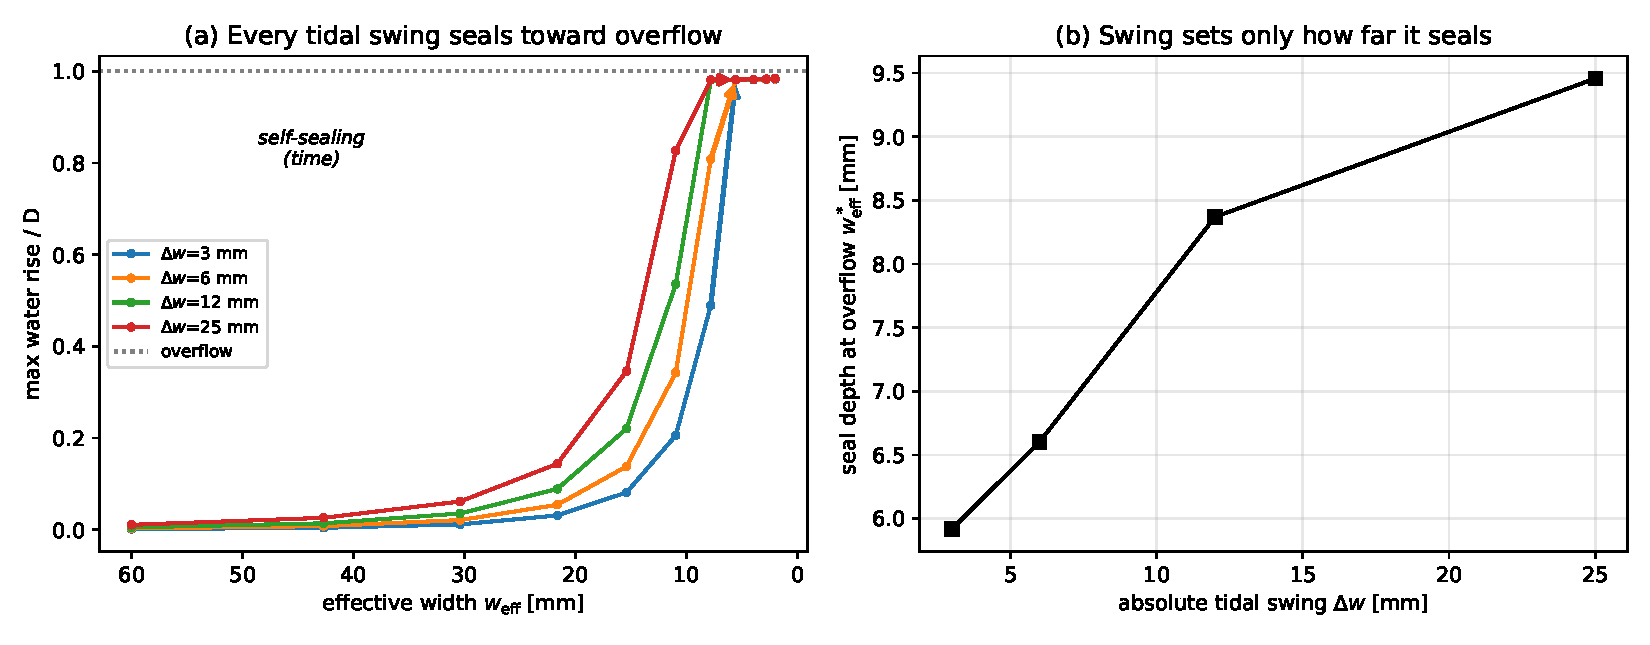
\includegraphics[width=0.95\textwidth]{Figures/wall_seal_regime.pdf}
    \caption{Self-sealing of the crack by wall condensation (effective-width model, equilibrium depth 5~km, surface $D=500$~m above the equilibrium water level). For a fixed absolute tidal swing $\Delta w=w_{\max}-w_{\min}$ of the walls, the ice lining lowers the mean width, i.e.\ the effective width $w_{\rm eff}$. (a) The maximum water rise (as a fraction of $D$) reaches overflow for every swing $\Delta w$ once the crack has sealed far enough --- there is no forcing threshold. (b) The swing sets only the seal depth $w_{\rm eff}^*$ at which overflow first occurs; it is of order millimetres and increases only weakly with the swing ($w_{\rm eff}^*\propto\Delta w^{0.3}$).}
    \label{fig:enc:seal}
\end{figure}

\subsection{Predicting the phase and strength of the two mass-flux peaks}
\label{sec:peaks}
Once the geometry is on the attractor, the diurnal mass flux is dominated by gas
evaporation $w\,\phi_{top}(w,\,D-h)$; the liquid overflow contributes less than
5\%. This flux has two peaks, both with a simple predictor.

The \emph{widening peak} occurs near the maximum-crack-width phase
(MA $\approx 180$--$215^\circ$, approaching $180^\circ$ for stronger forcing) and
its strength scales with the throughput there, $w_{\max}\,\phi_{top}(w_{\max},D-h_{180})$.
The \emph{approach peak} occurs near the maximum-water-level phase $\psi_h$
(MA $\approx 270$--$330^\circ$, with the flux maximum lying $\sim$10--40$^\circ$
earlier than $\psi_h$ because the width is already declining); its strength scales
with $w(\psi_h)\,\phi_{top}(w(\psi_h),\,D-h_{\max})$, and because $\phi_{top}$
rises steeply as the gas column shortens, it grows sharply as the water nears the
surface. The two peaks are therefore separated by $\psi_h-180^\circ\approx
90$--$140^\circ$, set by the forcing geometry.

The relative strength is governed by the closeness of approach $h_{\max}/D$ ---
the same attractor variable of Section~\ref{sec:attractor}
(Figure~\ref{fig:enc:peaks}). For a deep water table the widening peak dominates
and the approach peak is a weak secondary feature (or absent); as the sealing
drives $h_{\max}/D\to1$, the approach peak strengthens and overtakes the widening
peak. Thus the attractor not only produces a secondary peak but determines which
of the two is the main one. Identifying the stronger (approach) peak with the
observed main peak and the weaker (widening) peak with the secondary peak, and
allowing the single global phase offset the data permit, the predicted pair maps
onto main MA $180^\circ$ / secondary MA $\approx 50$--$60^\circ$, reproducing the
observed phase structure and the $\sim$130$^\circ$ separation.

\begin{figure}[hbt!]
    \centering
    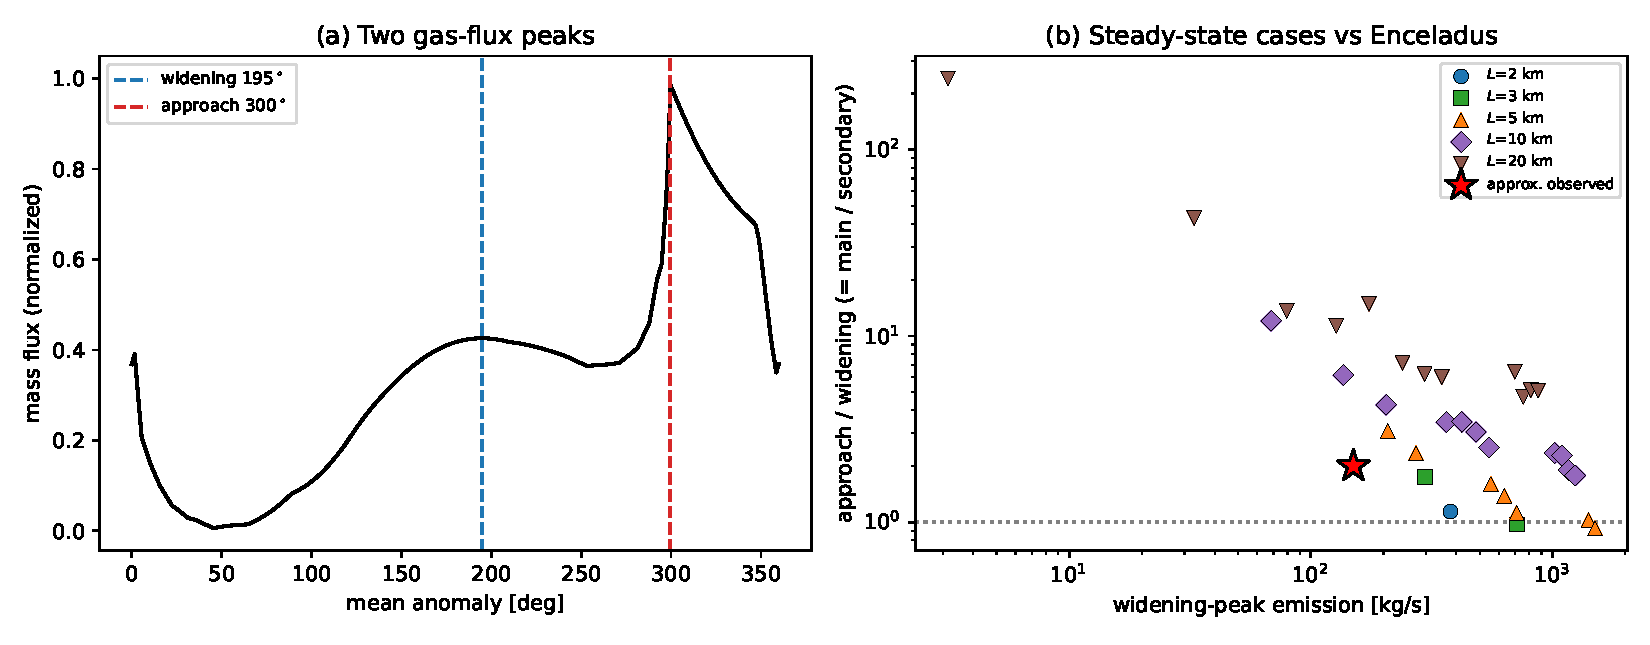
\includegraphics[width=0.95\textwidth]{Figures/peak_predictor.pdf}
    \caption{Predictor for the two diurnal mass-flux peaks (equilibrium depth
    5~km). (a) The gas-flux curve for a sealed crack ($\Delta w=10$~mm,
    $w_{\rm eff}=7$~mm) showing the widening peak near the max-width phase and the
    approach peak near the max-water-level phase. (b) The approach-to-widening
    strength ratio rises steeply with the closeness of approach $h_{\max}/D$ and
    crosses unity (approach becomes the main peak) as the sealing drives the
    water to the surface; curves are different absolute tidal swings $\Delta w$.}
    \label{fig:enc:peaks}
\end{figure}

\subsection{Comparison with the observed emission}
The model also reproduces the absolute magnitude of the plume. Multiplying the
diurnal mass flux per unit crack length by the $\sim$500~km summed length of the
tiger stripes \cite{spitale2007association}, representative attractor cases
(sealed to $w_{\rm eff}\sim$~mm, with the water reaching the surface) give a
cycle-mean total emission of $\sim$230--490~kg/s, in agreement with the
$200$--$400$~kg/s inferred from Cassini UVIS solar occultations
\cite{hansen2011composition,hansen2017investigation}. For the same cases the
secondary-to-main peak amplitude ratio is below unity, i.e.\ a weaker secondary
peak, consistent with the observed slab-density profile \cite{ingersoll2020time}.
Because the total scales linearly with the assumed active length, this magnitude
is an order-of-unity check rather than a tight constraint; conversely, the
secondary-to-main ratio depends on the absolute swing $\Delta w$ and the depth,
and could be inverted to constrain them.

\section{Conclusions}
We modeled the activities of the plumes on Enceladus by treating the crack as a long fissure whose walls widen and narrow over the diurnal cycle. The water level is strongly correlated with the rate of wall motion, and because friction makes the water-level excursion scale steeply with the inverse crack width, a narrowing crack drives the water toward the surface.

We noted that an active open crack is a more likely explanation of the observed variability than a closed one, as the warm walls are exposed only when the crack is open. Hence, the proposed model shows an additional evidence that the two-way mass exchange exists between the interior ocean and the planetary surface, which is important for the chemical energy sources for habitability \cite{parkinson2008habitability}.

We further argued that condensation of the plume onto the walls continually seals the crack, and that this self-sealing acts as an attractor: independent of its initial width, any crack that flexes is driven within a few diurnal cycles to a small-width state in which the water reaches the surface and produces the secondary peak. Because the ice lining lowers the mean width but leaves the absolute tidal swing of the walls unchanged, there is no forcing threshold for this overflow state to exist; the swing sets only how far the crack must seal first, and a sufficiently weak swing seals it to a residual gap so small that the plume becomes negligible. The narrow-width overflow regime is therefore a natural end-state rather than a fine-tuned configuration. On this attractor the diurnal mass flux carries two gas-evaporation peaks --- a widening peak near the maximum-width phase and an approach peak near the maximum-water-level phase --- whose phases and relative strength we predict from the forcing geometry and the closeness of approach; as the water nears the surface the approach peak overtakes the widening peak, and the pair reproduces the observed main / secondary peaks near MA $180^\circ$ and $50^\circ$. How the deposited ice is redistributed from the lip, through fracture and viscoelastic creep, remains an open problem that ultimately sets the long-term balance between sealing and the reopening maintained by the rising water.

While some assumptions are made, the physical processes modeled would follow a similar pattern. Future work can consider a more realistic geometry and generalize the model beyond the current assumptions. Considering an irregular shape of the crack would be possible, but it allows too high a degree of freedom for explorations in the parameter space. Also, the narrowing and widening of the crack may follow a different pattern, where the geometries and viscoelasticity can play a role. 


%%

%  Numbered lines in equations:
%  To add line numbers to lines in equations,
%  \begin{linenomath*}
%  \begin{equation}
%  \end{equation}
%  \end{linenomath*}



%% Enter Figures and Tables near as possible to where they are first mentioned:
%
% DO NOT USE \psfrag or \subfigure commands.
%
% Figure captions go below the figure.
% Acronyms used in figure captions will be spelled out in the final, published version.

% Table titles go above tables;  other caption information
%  should be placed in last line of the table, using
% \multicolumn2l{$^a$ This is a table note.}
% NOTE that there is no difference between table caption and table heading in the final, published version
%
%----------------
% EXAMPLE FIGURES
%
% \begin{figure}
% \includegraphics{example.png}
% \caption{caption}
% \end{figure}
%
% Giving latex a width will help it to scale the figure properly. A simple trick is to use \textwidth. Try this if large figures run off the side of the page.
% \begin{figure}
% \noindent\includegraphics[width=\textwidth]{anothersample.png}
%\caption{caption}
%\label{pngfiguresample}
%\end{figure}
%
%
% If you get an error about an unknown bounding box, try specifying the width and height of the figure with the natwidth and natheight options. This is common when trying to add a PDF figure without pdflatex.
% \begin{figure}
% \noindent\includegraphics[natwidth=800px,natheight=600px]{samplefigure.pdf}
%\caption{caption}
%\label{pdffiguresample}
%\end{figure}
%
%
% PDFLatex does not seem to be able to process EPS figures. You may want to try the epstopdf package.
%

%
% ---------------
% EXAMPLE TABLE
%
% \begin{table}
% \caption{Time of the Transition Between Phase 1 and Phase 2$^{a}$}
% \centering
% \begin{tabular}{l c}
% \hline
%  Run  & Time (min)  \\
% \hline
%   $l1$  & 260   \\
%   $l2$  & 300   \\
%   $l3$  & 340   \\
%   $h1$  & 270   \\
%   $h2$  & 250   \\
%   $h3$  & 380   \\
%   $r1$  & 370   \\
%   $r2$  & 390   \\
% \hline
% \multicolumn{2}{l}{$^{a}$Footnote text here.}
% \end{tabular}
% \end{table}

%%%%%%%%%%%%%%%%%%%%%%%%%%%%%%%%%%%%%%%%%%%%%%%
% SIDEWAYS FIGURES and TABLES
% AGU prefers the use of {sidewaystable} over {landscapetable} as it causes fewer problems.
%
% \begin{sidewaysfigure}
% \includegraphics[width=20pc]{figsamp}
% \caption{caption here}
% \label{newfig}
% \end{sidewaysfigure}
%
%  \begin{sidewaystable}
%  \caption{Caption here}
% \label{tab:signif_gap_clos}
%  \begin{tabular}{ccc}
% one&two&three\\
% four&five&six
%  \end{tabular}
%  \end{sidewaystable}

%% If using numbered lines, please surround equations with \begin{linenomath*}...\end{linenomath*}
%\begin{linenomath*}
%\begin{equation}
%y|{f} \sim g(m, \sigma),
%\end{equation}
%\end{linenomath*}

%%% End of body of article

%%%%%%%%%%%%%%%%%%%%%%%%%%%%%%%%%%%%%%%%%%%%%%%
%% Optional Appendices go here
%
% The \appendix command resets counters and redefines section heads
%
% After typing \appendix
%
%\section{Here Is Appendix Title}
% will show
% A: Here Is Appendix Title
%
%\appendix
%\section{Here is a sample appendix}

%%%%%%%%%%%%%%%%%%%%%%%%%%%%%%%%%%%%%%%%%%%%%%%
% Optional Glossary, Notation or Acronym section goes here:
%
% Glossary is only allowed in Reviews of Geophysics
%  \begin{glossary}
%  \term{Term}
%   Term Definition here
%  \term{Term}
%   Term Definition here
%  \term{Term}
%   Term Definition here
%  \end{glossary}


%%%%%%%%%%%%%%%%%%%%%%%%%%%%%%%%%%%%%%%%%%%%%%%
% Acronyms
%% NOTE that acronyms in the final published version will be spelled out when used in figure captions.
%   \begin{acronyms}
%   \acro{Acronym}
%   Definition here
%   \acro{EMOS}
%   Ensemble model output statistics
%   \acro{ECMWF}
%   Centre for Medium-Range Weather Forecasts
%   \end{acronyms}


%%%%%%%%%%%%%%%%%%%%%%%%%%%%%%%%%%%%%%%%%%%%%%%
% Notation
%   \begin{notation}
%   \notation{$a+b$} Notation Definition here
%   \notation{$e=mc^2$}
%   Equation in German-born physicist Albert Einstein's theory of special
%  relativity that showed that the increased relativistic mass ($m$) of a
%  body comes from the energy of motion of the body—that is, its kinetic
%  energy ($E$)—divided by the speed of light squared ($c^2$).
%   \end{notation}




%%%%%%%%%%%%%%%%%%%%%%%%%%%%%%%%%%%%%%%%%%%%%%%
%
% DATA SECTION and ACKNOWLEDGMENTS
%
%%%%%%%%%%%%%%%%%%%%%%%%%%%%%%%%%%%%%%%%%%%%%%%

\section*{Open Research Section}
This is a modelling study and uses no new observational data. The model source
code that produces all results and figures in this work --- the Python solver
(with an optional C++ performance core), the configuration files, and the
figure-generating scripts --- is openly available in the \texttt{EnceladusPlume}
repository at \url{https://github.com/cshsgy/EnceladusPlume}. The observed slab
density shown in Figure~\ref{fig:enc:1} is reproduced from \citeA{ingersoll2020time}.
% For final submission, deposit a versioned archive of the repository (e.g. Zenodo)
% and cite its DOI here, as AGU requires an archived, citable data/software record.

\section*{As Applicable – Inclusion in Global Research Statement}
The Authorship: Inclusion in Global Research policy aims to promote greater equity and transparency in research collaborations. AGU Publications encourage research collaborations between regions, countries, and communities and expect authors to include their local collaborators as co-authors when they meet the AGU Publications authorship criteria (described here: https://www.agu.org/publications/authors/policies\#authorship). Those who do not meet the criteria should be included in the Acknowledgement section. We encourage researchers to consider recommendations from The TRUST CODE - A Global Code of Conduct for Equitable Research Partnerships (https://www.globalcodeofconduct.org/) when conducting and reporting their research, as applicable, and encourage authors to include a disclosure statement pertaining to the ethical and scientific considerations of their research collaborations in an “Inclusion in Global Research Statemstandalone section in the manuscript following the Conclusions section. This can include disclosure of permits, authorizations, permissions and/or any formal agreements with local communities or other authorities, additional acknowledgements of local help received, and/or description of end-users of the research. You can learn more about the policy in this editorial. Example statements can be found in the following published papers: 
Holt et al. (https://agupubs.onlinelibrary.wiley.com/doi/full/10.1029/2022JG007188), 
Sánchez-Gutiérrez et al. (https://agupubs.onlinelibrary.wiley.com/doi/abs/10.1029/2023JG007554), 
Tully et al. (https://agupubs.onlinelibrary.wiley.com/doi/epdf/10.1029/2022JG007128) 
Please note that these statements are titled as “Global Research Collaboration Statements” from a previous pilot requirement in JGR Biogeosciences. The pilot has ended and statements should now be titled “Inclusion in Global Research Statement”.

\section*{Conflict of Interest declaration}
Please include a comprehensive conflict of interest statement that reflect all conflicts of interest for all involved authors. If there are no conflicts of interest please state, “The authors declare there are no conflicts of interest for this manuscript.”



\acknowledgments
Enter acknowledgments here. This section is to acknowledge funding, thank colleagues, enter any secondary affiliations, and so on.


\bibliography{enceladus}



%Reference citation instructions and examples:
%
% Please use ONLY \cite and \citeA for reference citations.
% \cite for parenthetical references
% ...as shown in recent studies (Simpson et al., 2019)
% \citeA for in-text citations
% ...Simpson et al. (2019) have shown...
%
%
%...as shown by \citeA{jskilby}.
%...as shown by \citeA{lewin76}, \citeA{carson86}, \citeA{bartoldy02}, and \citeA{rinaldi03}.
%...has been shown \cite{jskilbye}.
%...has been shown \cite{lewin76,carson86,bartoldy02,rinaldi03}.
%... \cite <i.e.>[]{lewin76,carson86,bartoldy02,rinaldi03}.
%...has been shown by \cite <e.g.,>[and others]{lewin76}.
%
% apacite uses < > for prenotes and [ ] for postnotes
% DO NOT use other cite commands (e.g., \citeA, \cite, \citeyear, \nocite, \citealp, etc.).
%



\end{document}



More Information and Advice:

%%%%%%%%%%%%%%%%%%%%%%%%%%%%%%%%%%%%%%%%%%%%%%%
%
%  SECTION HEADS
%
%%%%%%%%%%%%%%%%%%%%%%%%%%%%%%%%%%%%%%%%%%%%%%%

% Capitalize the first letter of each word (except for
% prepositions, conjunctions, and articles that are
% three or fewer letters).

% AGU follows standard outline style; therefore, there cannot be a section 1 without
% a section 2, or a section 2.3.1 without a section 2.3.2.
% Please make sure your section numbers are balanced.
% ---------------
% Level 1 head
%
% Use the \section{} command to identify level 1 heads;
% type the appropriate head wording between the curly
% brackets, as shown below.
%
%An example:
%\section{Level 1 Head: Introduction}
%
% ---------------
% Level 2 head
%
% Use the \subsection{} command to identify level 2 heads.
%An example:
%\subsection{Level 2 Head}
%
% ---------------
% Level 3 head
%
% Use the \subsubsection{} command to identify level 3 heads
%An example:
%\subsubsection{Level 3 Head}
%
%---------------
% Level 4 head
%
% Use the \subsubsubsection{} command to identify level 3 heads
% An example:
%\subsubsubsection{Level 4 Head} An example.
%
%%%%%%%%%%%%%%%%%%%%%%%%%%%%%%%%%%%%%%%%%%%%%%%
%
%  IN-TEXT LISTS
%
%%%%%%%%%%%%%%%%%%%%%%%%%%%%%%%%%%%%%%%%%%%%%%%
%
% Do not use bulleted lists; enumerated lists are okay.
% \begin{enumerate}em
% \item
% \end{enumerate}
%
%%%%%%%%%%%%%%%%%%%%%%%%%%%%%%%%%%%%%%%%%%%%%%%
%
%  EQUATIONS
%
%%%%%%%%%%%%%%%%%%%%%%%%%%%%%%%%%%%%%%%%%%%%%%%

% Single-line equations are centered.
% Equation arrays will appear left-aligned.

Math coded inside display math mode \[ ...\]
 will not be numbered, e.g.,:
 \[ x^2=y^2 + z^2\]

 Math coded inside \begin{equation} and \end{equation} will
 be automatically numbered, e.g.,:
 \begin{equation}
 x^2=y^2 + z^2
 \end{equation}


% To create multiline equations, use the
% \begin{eqnarray} and \end{eqnarray} environment
% as demonstrated below.
\begin{eqnarray}
  x_{1} & = & (x - x_{0}) \cos \Theta \nonumber \\
        && + (y - y_{0}) \sin \Theta  \nonumber \\
  y_{1} & = & -(x - x_{0}) \sin \Theta \nonumber \\
        && + (y - y_{0}) \cos \Theta.
\end{eqnarray}

%If you don't want an equation number, use the star form:
%\begin{eqnarray*}...\end{eqnarray*}

% Break each line at a sign of operation
% (+, -, etc.) if possible, with the sign of operation
% on the new line.

% Indent second and subsequent lines to align with
% the first character following the equal sign on the
% first line.

% Use an \hspace{} command to insert horizontal space
% into your equation if necessary. Place an appropriate
% unit of measure between the curly braces, e.g.
% \hspace{1in}; you may have to experiment to achieve
% the correct amount of space.


%%%%%%%%%%%%%%%%%%%%%%%%%%%%%%%%%%%%%%%%%%%%%%%
%
%  EQUATION NUMBERING: COUNTER
%
%%%%%%%%%%%%%%%%%%%%%%%%%%%%%%%%%%%%%%%%%%%%%%%

% You may change equation numbering by resetting
% the equation counter or by explicitly numbering
% an equation.

% To explicitly number an equation, type \eqnum{}
% (with the desired number between the brackets)
% after the \begin{equation} or \begin{eqnarray}
% command.  The \eqnum{} command will affect only
% the equation it appears with; LaTeX will number
% any equations appearing later in the manuscript
% according to the equation counter.
%

% If you have a multiline equation that needs only
% one equation number, use a \nonumber command in
% front of the double backslashes (\\) as shown in
% the multiline equation above.

% If you are using line numbers, remember to surround
% equations with \begin{linenomath*}...\end{linenomath*}

%  To add line numbers to lines in equations:
%  \begin{linenomath*}
%  \begin{equation}
%  \end{equation}
%  \end{linenomath*}




